% We choose the style and text-size.
\documentclass[%
  final,  % Set to draft instead of final to speed-up compile time
  12pt,  % If not conforming to a strict character, use 11pt
  british,
  a4paper
]{article}

% Packages we load
\usepackage[utf8]{inputenc}
\usepackage[T1]{fontenc}
\usepackage{geometry}
\usepackage{graphicx}
\usepackage{hyperref}
\hypersetup{
    colorlinks=true, % Aktivér farvede links
    linkcolor=black, % Farve på links (til kapitler, sektioner osv.)
    citecolor=black, % Farve på citations-links
    urlcolor=black   % Farve på URL-links
}
\usepackage{enumitem}
\usepackage{setspace}
\usepackage{titlesec}
\usepackage{tabularx}
\usepackage{booktabs}
\usepackage{caption}
\usepackage{float}
\usepackage{array}
\usepackage{listings}
\usepackage{xcolor}
\usepackage{amsmath}



% Ny kommando der laver fine linjer (\NL)
\newcommand{\NL}{\vspace{1em}\noindent} 

\lstset{
    language=R,
    basicstyle=\ttfamily\small,
    keywordstyle=\bfseries,
    commentstyle=\itshape,
    stringstyle=\ttfamily,
    breaklines=true,
    frame=single,
    columns=fullflexible,
    showstringspaces=false
} % Used to insert R code.

% Margins
\geometry{margin=2.5cm}
\setstretch{1.2}

%\makeatletter
%\renewcommand{\@fnsymbol}[1]{\arabic{#1}}
%\makeatother

% Define a title here
\title{\textbf{DAM Assignment 1-4}}
\author{
Jonas Hougaard\\
Rose Marie N. Ore\\
Johan K. Eskildsen \\
Søren L.F. Lageri\footnote{All authors of the Digital Archives and Methods assignments included in this document collaborated on and solved the work jointly. Therefore, they are listed here rather than individually throughout the assignments.}
}
\date{\today}

% Here the document begins
\begin{document}

\maketitle

\section*{Part 1: Regex and OpenRefine}

\textbf{Task 1:} List regex that extracts dates from \url{http://bit.ly/regexexercise2} and formats them as YYYY-MM-DD?

\NL\textbf{URL for the solution:} \url{https://regex101.com/r/dd3e1R/1}

\NL\textbf{Brief explanation:} The text included dates with whitespace in front of both the year and the month. Therefore, we needed to search for all possible instances which had a whitespace and the ones that did not and this was done by utilising \textbackslash s?

The final search was therefore: \textnormal{(\textbackslash d\{1,2\}).\textbackslash s?(\textbackslash d\{1,2\}).\textbackslash s?(\textbackslash d\{4\})}

\NL By using the parentheses, we could separate them into three groups, where group one was the day, group two was the month, and group three was the year. Lastly, we used the substitution function and inserted \$3-\$2-\$1, where the dash separates the groups. We got a new reconstructed text where the dates had the desired format of YYYY-MM-DD. \newline

\noindent\textbf{Task 2:} Regex to convert stopwordlist between R and Voyant format

\NL\textbf{URL for the solution:} \url{https://regex101.com/r/dd3e1R/2/substitution}

\NL\textbf{Voyant to R}

\noindent\textbf{Brief explanation:} We used the regular expression: \textbackslash n in regex101. This means that it found the invisible character marking where a new line started. Then we went to “substitution” in regex101 and typed: (","). This means that it replaces the line breaks with commas by inserting: “,”
This way all line breaks became commas and this way we got a neat stopwordlist that works in R. It looks like this:

\begin{figure}[ht]
    \centering
    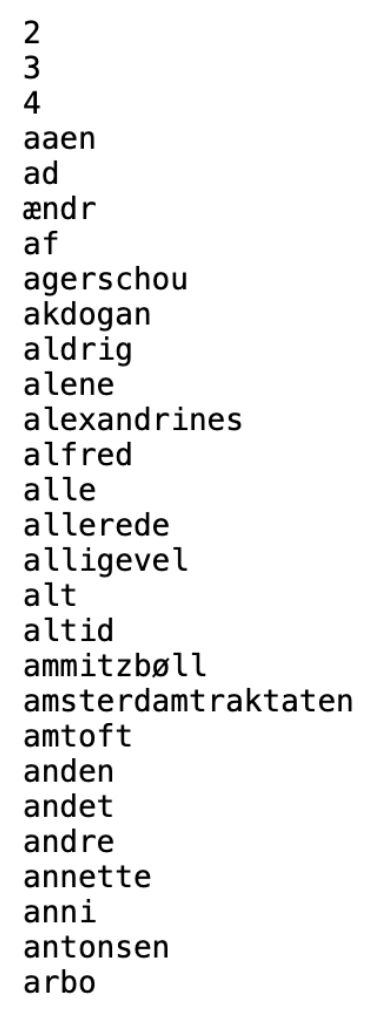
\includegraphics[width=1\linewidth]{images/task2.a.png}
    \caption{Regex expression to convert stopwordslist from Voyant to R.}
    \label{fig:task2a}
\end{figure}

It can be noted that only a handful of the stopwordlist is shown here. Also, the first and last words manually need to have a quotation mark (“) added.

\NL\textbf{R to Voyant}

\NL\textbf{Brief explanation:} 

In order to convert a stopwordlist that was in the format of R to a format that was usable in Voyant we did the following. First we wrote this code in R to create a stopwordslist.

\begin{verbatim}
    stopwords <- c(“2”,”3”,"...”,”wilhjelm”,”yildiz”)
\end{verbatim}

Where the “…” indicates all of the other stopwords within the list, which are excluded here to keep it tidy.
Afterwards, we wrote the following code, which created a text file, that is compatible with Voyant.

\begin{verbatim}
    writeLines(stopwords, "stopwords.txt")
\end{verbatim}

\noindent Lastly, we wanted R to show us the list and we did that with the following code.

\begin{verbatim}
    file.show("stopwords.txt")
\end{verbatim}

\noindent That returned the following image from R.

\begin{figure}[ht]
    \centering
    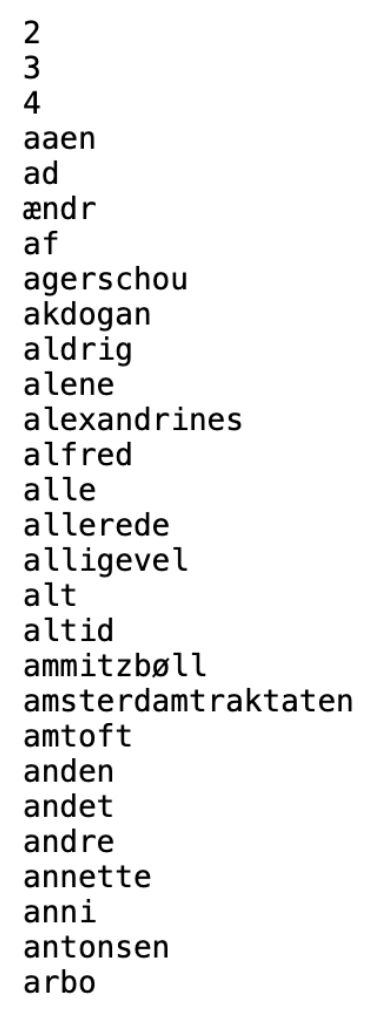
\includegraphics[width=0.3\linewidth]{images/task2.b.png}
    \caption{Stopwordslist created with R to be used in Voyant.}
    \label{fig:task2b}
\end{figure}

Only a handful of the words are shown in Figure \ref{fig:task2b} but it still shows that the format was indeed suited for Voyant.\newline

\noindent\textbf{Task 3:} Does OpenRefine alter the raw data during sorting and filtering?

YES/\textbf{NO}

\noindent\textbf{Answer}

No, OpenRefine does not alter the raw data. OpenRefine uses the data as a “template” but any changes made do not affect the original uploaded data-file. We would always want to keep our raw data stored in case something went wrong with the data analysis or someone else wants to recreate the data-analysis. Therefore, the raw data should always be available to others. \newline

\noindent\textbf{Task 4:} Which two months are reported as the most water-deprived/driest?

\NL\textbf{Answer:} We based the two most water deprived months on the variable “months\_no\_water” as we believed the months with no water must be the most water-deprived. 

We started by reordering the columns so the variable “months\_no\_water” was the third column in the table. This was done by selecting the drop-down arrow next to All, Edit Columns, Re-order/remove columns…, holding down the mouse button and dragging the variable to the second row.

Next, we transformed the column by clicking the drop-down arrow next to the column name, then Edit cells, and Transform. We wanted to remove the square brackets (“[ ]”), the quotation marks (‘), and the empty spaces (“ “) from the cells. Therefore, we wrote the following expression: 

\begin{verbatim}
    value.replace("[","").replace("]","").replace("’","").replace(" ",""). 
\end{verbatim}

\noindent Next, we wanted to split the values within the cells from each other, since there were multiple months in the same cell. Therefore, we again selected the drop-down arrow, Edit cells, Split multi-valued cells, ... 

Since the values are separated by a semicolon (;), we wrote this as the separator and pressed OK. Lastly, we wanted to see the amount of times the months were mentioned, so we selected the drop-down arrow, Facet, and Text facet.

\begin{figure}[ht]
    \centering
    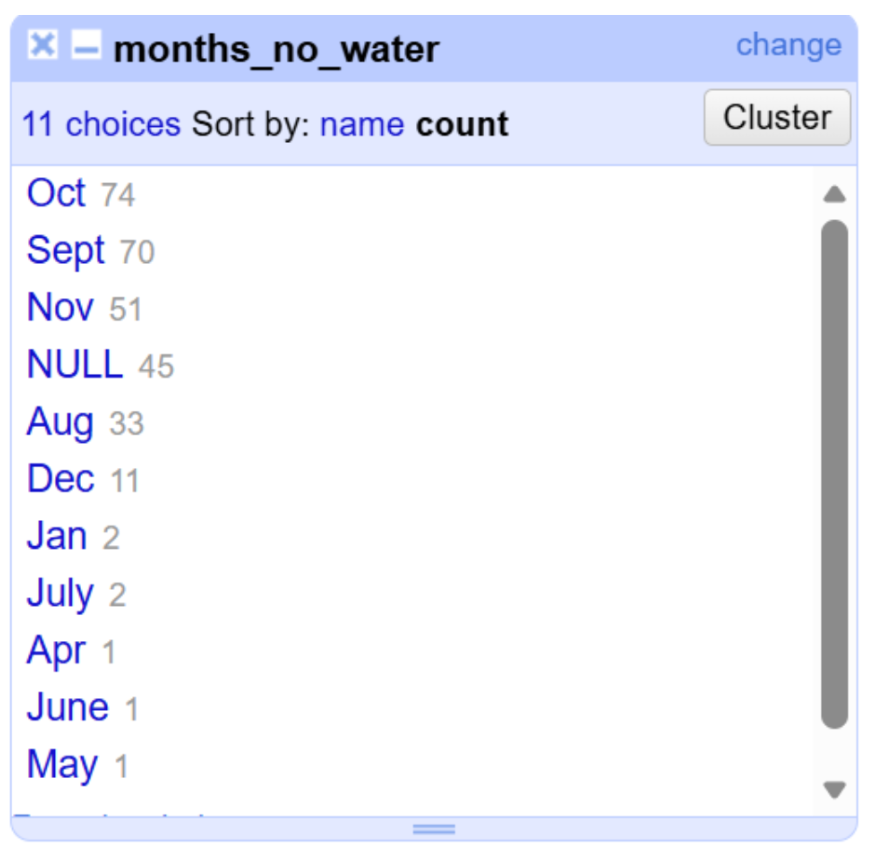
\includegraphics[width=0.5\linewidth]{images/task4.png}
    \caption{The two months which were most water-deprived/driest by the interviewed farmer households}
    \label{fig:task4}
\end{figure}

By looking at Figure \ref{fig:task4} we could see that October is the most water deprived month with it being mentioned 74 times and September is the second most water deprived month, being mentioned 70 times.\newline

\noindent\textbf{Task 5:} 10 most common occupations in 1801 Aarhus.

\begin{itemize}
    \item \textbf{Total number of people in your selected cohort:} 2244
    \item \textbf{Define what is/is not an occupation:} You could argue that “invalid”,  “arbejdsløs” and “lever af sine midler”  are not occupations but since the dataset has put it as an occupation we have chosen to keep it as such. There were also two entries with unknown gender, which were left blank, and can be seen in Figure \ref{fig:task5b}. We could not be certain about the gender of the two instances so we chose to exclude those two from the data analysis.
\end{itemize}

We chose to focus on women for this assignment. We moved all the relevant columns up, which were koen (gender), alder (age), civilstand (marital status) and erhverv (occupation). Then we clicked on text facet on gender and marital status and chose to only show women and unmarried. Then we went to edit cells in the “age” column, then clicked common transforms and then “to number”, to make sure that the program knows that the digits we are working with are numbers and in this instance age. Then we clustered the cells in the occupations column as much as possible by using the cluster function. 

Many of the descriptions of the same occupations had varieties that we afterwards manually fixed by editing the names into categories with the same name. For instance, we made a category called “Skrædderpige”, in which we included cells with names such as “syer”, “nærer sig ved syening”, “syerske”. This resulted in the following Figure.

\begin{figure}[ht]
    \centering
    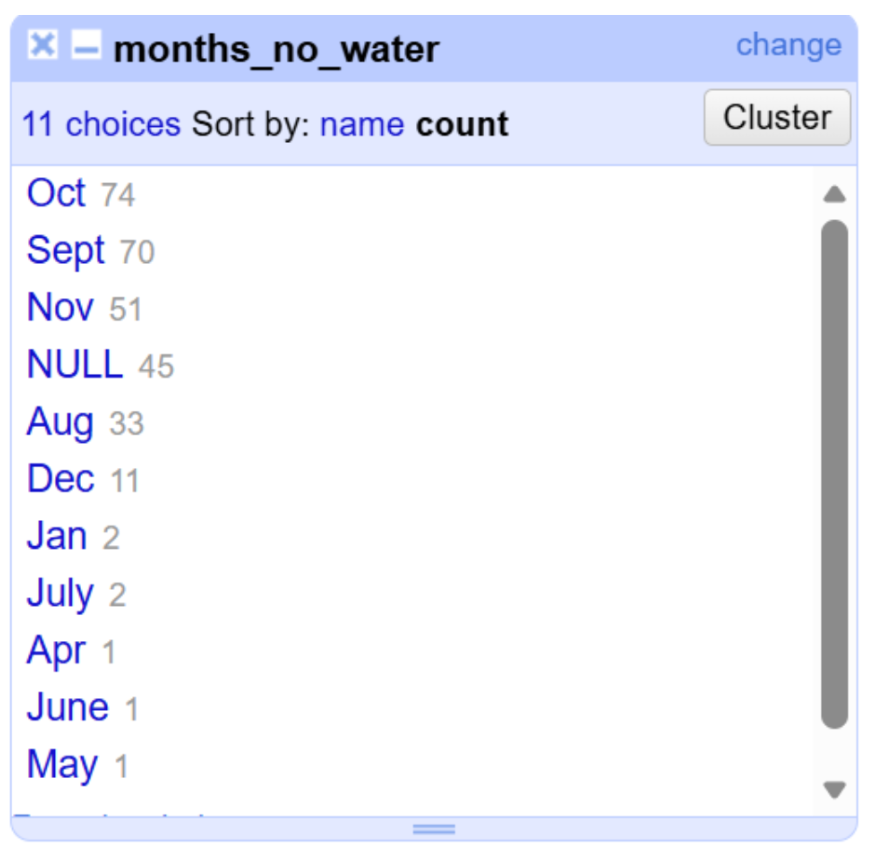
\includegraphics[width=1\linewidth]{images/task5.a.png}
    \caption{The top ten most frequent occupations for women between the ages of 20-30 in 1801 Aarhus.}
    \label{fig:task5a}
\end{figure}

\begin{figure}[ht]
    \centering
    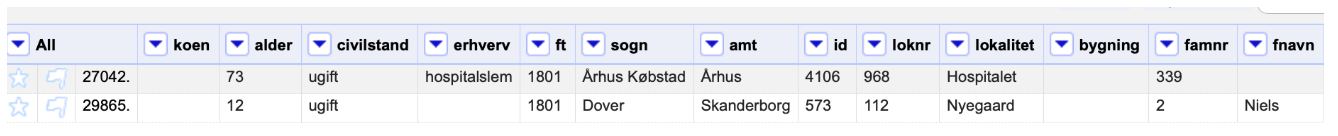
\includegraphics[width=1\linewidth]{images/task5.b.png}
    \caption{The two unknown genders and their occupations.}
    \label{fig:task5b}
\end{figure}
\clearpage
\textbf{10 most frequent occupations:}
\begin{enumerate}[]
    \item Tjenestepige (Maid)
    \item Væverske (Weaver)
    \item Skrædderpige (Tailor)
    \item Husholderske (Housekeeper)
    \item invalid (Invalid/Disabled)
    \item Spinderske (Spinning)
    \item Tigger/arbejdsløs (Beggar/Unemployed)
    \item Inderste (Innermost)
    \item Lever af sine midler (Living of their funds)
    \item Kokkepige (Cook)
\end{enumerate}

\newpage

\section*{Part 2: Danish Monarchs}

\textbf{Github URL:} 

\noindent\href{https://github.com/Digital-Methods-HASS/AU754395_Lageri_Soeren/tree/main/week11}{AU754395\_Lageri\_Soeren/week11 at main · Digital-Methods-HASS/AU754395\_Lageri\_Soeren} 

\subsection*{Question 1}
What function did you use to load your dataset as a tibble?

\textbf{Code:}
\begin{lstlisting}
library(tidyverse)

kings <- read_csv2("../week11/kings.csv")

find("read.csv") # Returns "package:utils"
find("read_csv") # Returns "package:readr"
\end{lstlisting}

\textbf{Answer:}
From the start of the document, where we loaded the \verb|tidyverse| library, we can see that the package \verb|readr| is a part of \verb|tidyverse|. Therefore, \verb|read_csv| and \verb|read_csv2| are \verb|tidyverse| functions. Meanwhile, the \verb|utils| package is a part of the base-R packages.

Objects created with \verb|.csv| and \verb|_csv| place all variables within the first column because the separator is not interpreted correctly.
But by using \verb|.csv2| and \verb|_csv2| the variables are separated to be within their own respective column, since R interprets semi colon (;) to be the delimiter, which separates the columns.
Generally, when extracting a single column from a tibble, the tibble will remain a tibble, whereas a data frame becomes a vector when you extract a single column from it. Therefore, for our case we will stay with tibbles and use the kings4 dataset, which utilizes the \verb|read_csv2| function from \verb|tidyverse|, since our dataset has semi colon (;) as the separator.

\subsection*{Question 2}
Average age of reign and how many exceeded it.

We want to define a new column that subtracts the end of the era with the start. We also want to keep rows where Era\_start has no \verb|NA| OR Era\_finished has no NA. This results in rows where both values are \verb|NA| being removed.
\clearpage
\textbf{Code:}

\begin{lstlisting}
# Pipes (%>%) are used to combine multiple functions.
# Filter out NA. (not necessary for us since we do not have any NA data.)
# Create a new column called "Reign_duration"

Reign_duration <- kings4 %>%
  filter(!is.na(Era_start) | !is.na(Era_finished)) %>% 
  mutate(Reign_duration = Era_finished - Era_start) 
    
Reign_duration[12] # The duration column is the 12th column and has 57 values.

Average_reign_duration_baseR <- 
  mean(as.numeric(Reign_duration$Reign_duration),na.rm = TRUE)

# cat functions do not work with pipes, so we type it separately.
# We round it to one digit.
cat("Base-R mean:",round(Average_reign_duration_baseR,digits=1),"years")

# Takes mean of the duration of the reigns and remove NA.
Average_reign_duration <- Reign_duration %>%
  summarize(avg_duration = mean(Reign_duration, na.rm = TRUE))

# The new tibble has one element at [1,1]
Average_reign_duration[1,1]

# Now we find the longer-than-average duration of reign.
# The $ extracts the avg_duration column from the Average_rule_duration tibble.
# We filter and select the four desired columns.

longer_than_avg_reigns <- Reign_duration %>%
  filter(Reign_duration > Average_reign_duration$avg_duration) %>% 
  select(Name,Era_start,Era_finished,Reign_duration) 

# Lastly, we count the amount of elements
count(longer_than_avg_reigns)
\end{lstlisting}

\textbf{Result/Answer:}

\noindent \textbf{Base-R mean:} 19.3 years

\noindent Using \verb|tidyverse|, the \textbf{average duration (mean)} of the rulers was 19.3 years.

We get the same result but the benefit of using \verb|tidyverse| instead of the Base-R functions is that the result remains a tibble and does not become a vector. This can hence be used to filter which reigns were longer than the average reign.

\noindent There are \textbf{26 kings} who had a longer-than-average duration of reign.

\subsection*{Question 3}
How many days did the three longest-ruling monarchs rule?

\textbf{Code:}

\begin{lstlisting}
# First it arranges from biggest to smallest.
# Then it selects the first three rows.
# Makes new column and converts years to days (with leap).
# Lastly, select column 1, 12 and 13.

three_longest_reigns_days_optimised <- Reign_duration %>%
  arrange(desc(Reign_duration)) %>%
  slice(1:3) %>%
  mutate(Reign_days = Reign_duration*365.25) %>% 
  select(Name, Reign_duration, Reign_days)

three_longest_reigns_days_optimised
\end{lstlisting}

\textbf{Result/Answer:}

\noindent The three longest-ruling monarchs were:
\begin{itemize}
    \item Christian 4. with a reign of 60 years or 21915 days
    \item Margrethe 2. with a reign of 52 years or 18993 days
    \item Erik 7. af Pommern with a reign of 43 years or 15705.75 days
\end{itemize}

\subsection*{Question 4}
Plot duration of reign over time. What is the long-term trend in the duration of reign among Danish monarchs? How does it relate to the historical violence trends ? 

We first make a new column called \verb|midyear_Reign| to act as datapoints for our $x$-axis.

$$\text{midyear}=\text{Era\_start} + \frac{(\text{Era\_finished}-\text{Era\_start})}{2}$$

\clearpage
\textbf{Code:}
\begin{lstlisting}
midyear_Reign <- Reign_duration %>% 
  mutate(midyear = Era_start + (Era_finished-Era_start)/2)

ggplot(midyear_Reign, aes(x=midyear,y=Reign_duration)) +
  geom_point() + # gives data points in the plot
  geom_smooth() + # Fits a curve to the points.
  labs(
    title = "Duration of Danish Monarchs' Reigns Through Time",
    x = "Midyear of Reign",
    y = "Duration of Reign (years)"
  ) +
  theme_bw() +
  theme(text = element_text(size = 14))

ggsave("Duration of Danish Monarchs' Reigns Through Time.png" , width=14, height = 10, dpi=100)
\end{lstlisting}

\textbf{Visual:}

\begin{figure}[ht]
    \centering
    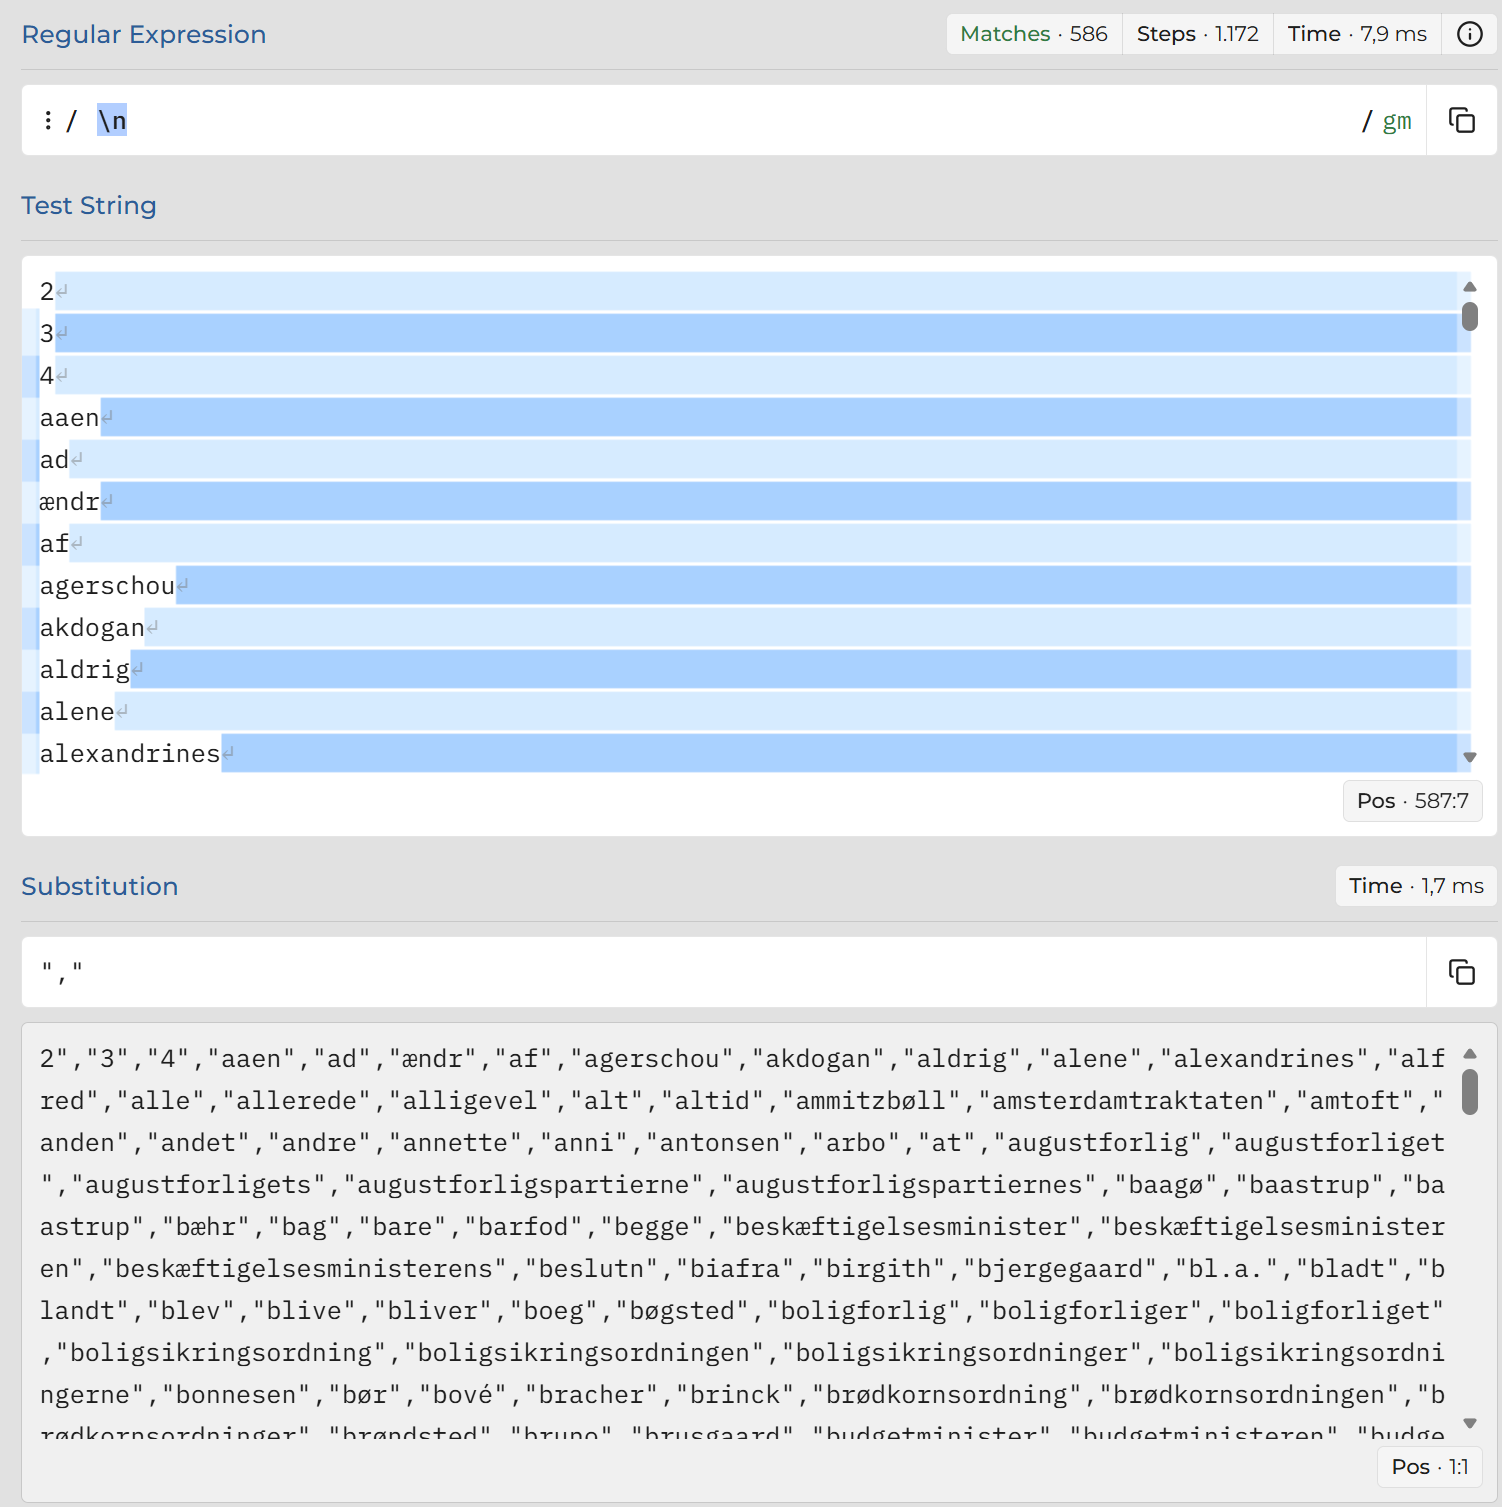
\includegraphics[width=\linewidth]{images/Duration of Danish Monarchs' Reigns Through Time.png}
    \caption{Visual created with $\textit{ggplot()}$ which shows the duration of Danish Monarchs' reigns through time.}
    \label{fig:kings_plot}
\end{figure}

\textbf{Answer:}

The plot in Figure \ref{fig:kings_plot} shows a blue line which is fitted to the data. Since it rises, we can conclude, that the average duration of the Danish Monarchs' reigns increases i.e. they generally rule for longer periods over time since they live longer.

Since we know there were still wars throughout the history of the Danish Monarchy, it is hard to make a direct connection between the historical period being less violent. However, one could make the assumption that a longer rule equals a more peaceful period but this could also be caused by advances in medicine and hygiene.

%\newpage

\section*{Part 3: Visualisation Assignment}

\noindent\textbf{Github URL:} 

\noindent \url{https://github.com/Digital-Methods-HASS/AU754395_Lageri_Soeren/tree/main/week13}

\subsection*{Visualisation}

\begin{figure}[ht] % You can add [H] so it becomes {figure}[H]. To place it "here"
    \centering
    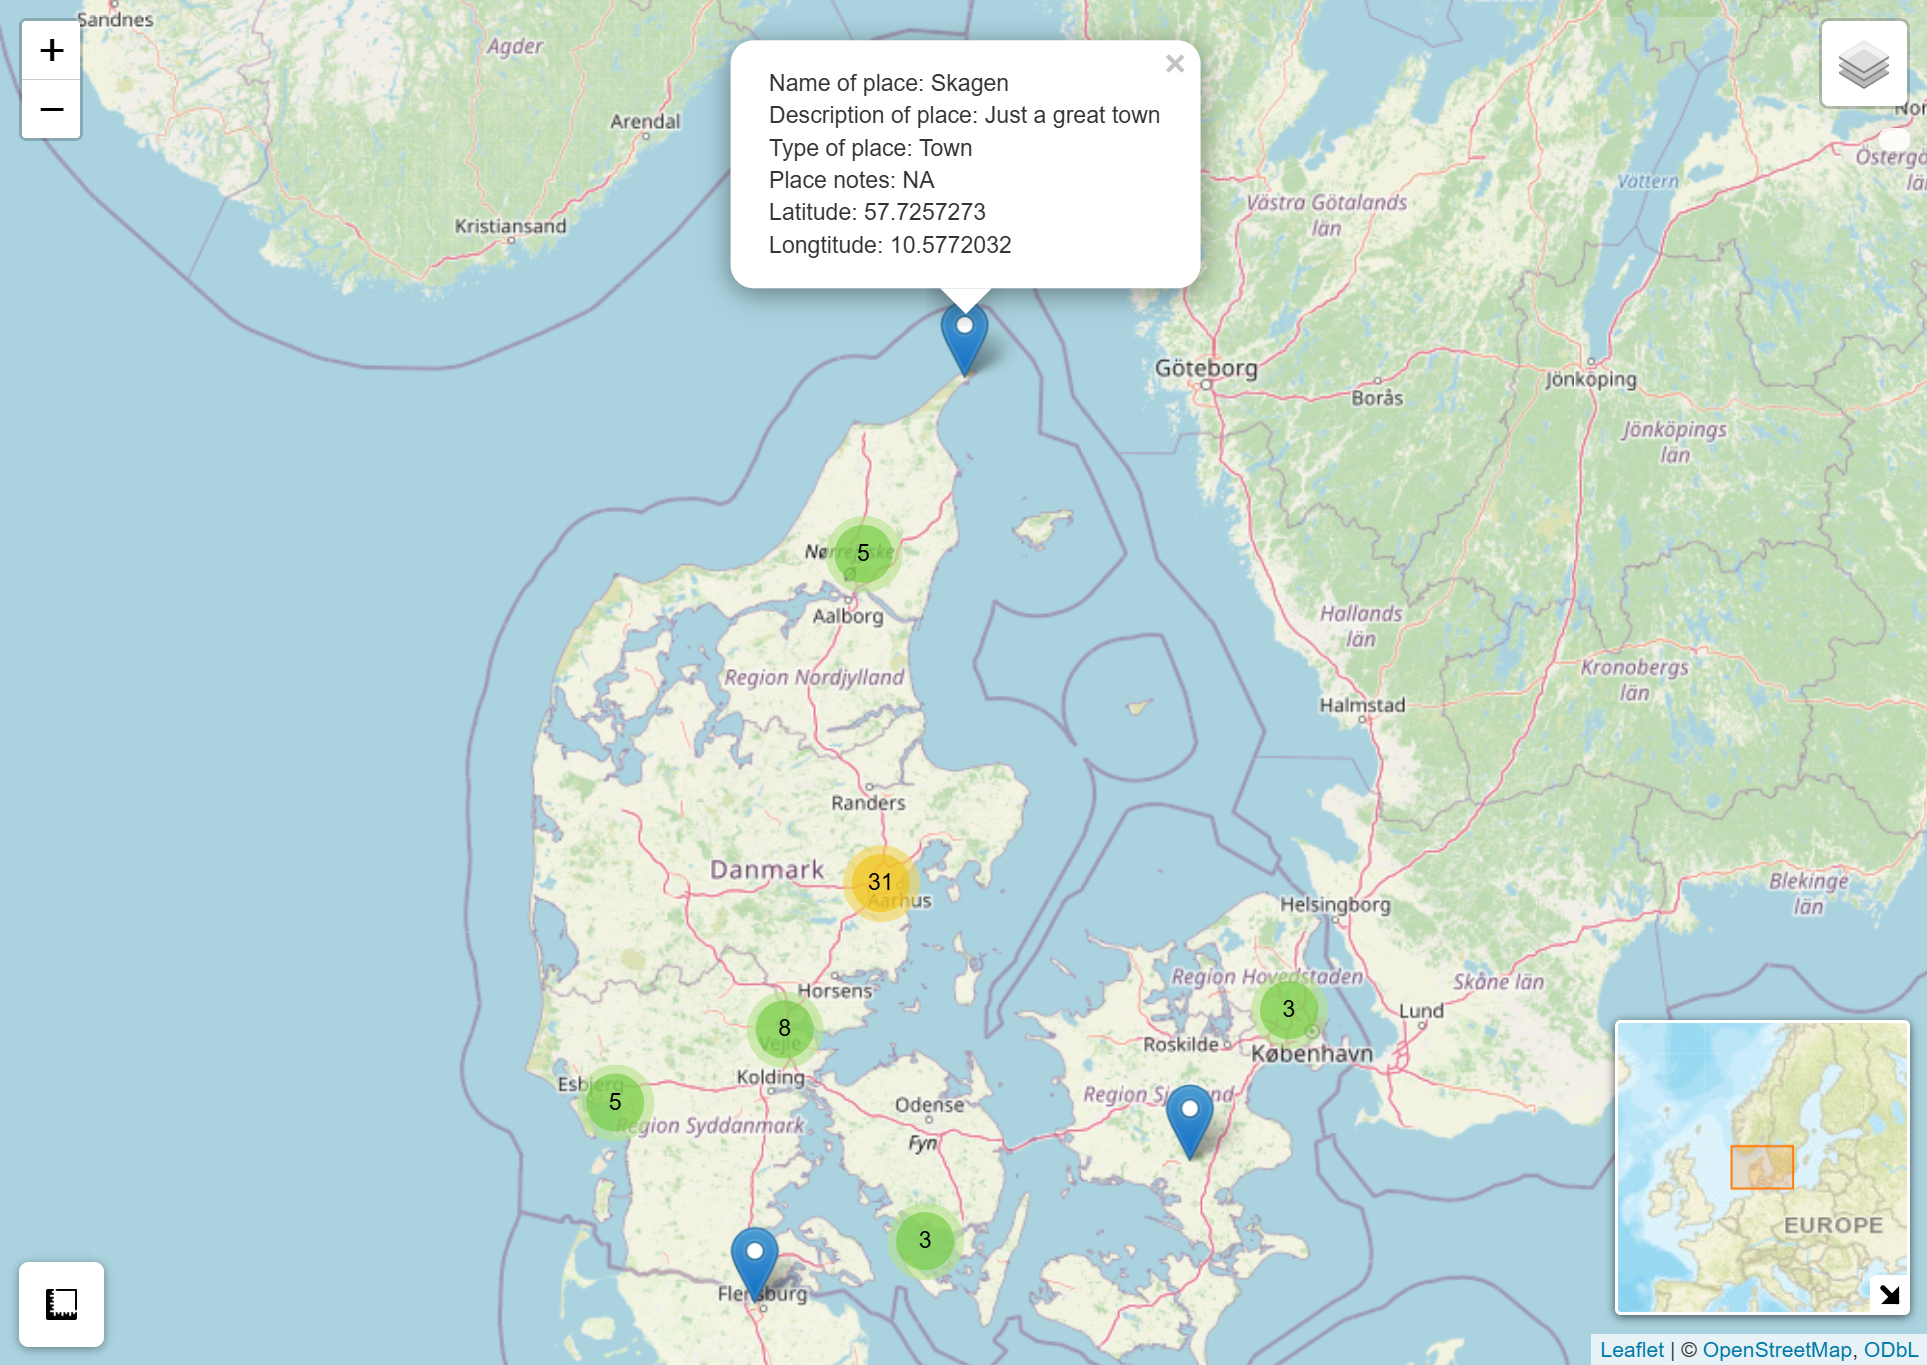
\includegraphics[width=\textwidth]{images/visual.png} % Change to .png or .jpg
    \caption{Map of Denmark with a collection of leisure places or places marked, which are collected in clusters.}
    \label{fig:visual} % define a nickname for your plot. Used to reference it
\end{figure}
\hspace{-0.5cm}
\subsection*{Significance}
\textbf{Explain what your visualisation represents and its implications ($\approx$ 250 words).}

\noindent The visualisation in Figure \ref{fig:visual} shows a map of Denmark, where we have used the coordinates from a selection of leisure places or places, to mark these according to where they can be found in Denmark. Each mark on the map contains the name of the place, a description of the place, what type they are, extra notes regarding the place and the coordinates for the place. The coordinates are separated into latitude and longitude respectively. Looking at Figure \ref{fig:visual} we used the marker \textit{Skagen}, which is the town closest to the tip of Denmark, to demonstrate the information the marker shows. This location also makes it possible for us to still see the 31 leisure places located around the city of Aarhus. 

The map from Figure \ref{fig:visual} shows that a large collection of leisure places is located within and around Aarhus. Since the leisure places were collected by students studying in Aarhus, it thereby makes sense that the majority of locations by students are situated in this area. It can also be assumed that this is also a causality of students living in Aarhus and thereby making it be more natural to know about the local specialities within Aarhus. Using cluster maps is a great way to bundle leisure places together making a comparison such as this possible.

\section*{Part 4: Digital archives reflection assignment}

\noindent\textbf{Part 1}

\noindent Jensen's category of digital archival literacy addresses the distinct challenges digital archives represent for historical research. Our first point of focus is that there has been a shift in medium from analogue to digital, which presents a new set of logics for use of historical sources. The quality of research now depends on the historians’ understanding of these logics. There’s a new set of search tools in digital archives that scholars use, which have their own logics, which are new for historians and which they need to understand to make high quality research. 

Our second point of focus is that digitization has changed the way historians interact with their sources. In a traditional archive all historical sources are preserved and shown in an equal manner, which can be seen here: “Still, most archival institutions make all sources available on equal terms if they are included in their collections.”\footnote{Jensen, Helle Strandgaard (2020), “Digital Archival Literacy for (all) Historians”, p. 4,  \textit{Media History}.} This changes when historians interact with digital sources because they have a tendency to make already-popular sources more widely available. Historians thus need to consider what they are not going to find online and how that will affect their work. They also need to consider what the goals and aims of digital archives are. They need to secure funding and therefore, they have to focus on getting the highest number of users to show sponsors a tangible output. This might affect what gets digitized, and historians need to be aware of this bias.
research.\newline

\noindent\textbf{Part 2.1}

\noindent The interviewee is the governmental administrator, Abraham Schramack. Schramack was a prominent figure in the French Third Republic, and he held different positions such as member of senate, minister of interior, head of national police etc. It is clear he held some important offices and must have been quite respected in the French political life. When Germany invaded France he managed to escape with the help of friends. He died in 1948. 

The source is a recording from August 21, 1946, of an interview made by David Boder, and is part of a group of interviews of the Kahn family. The description-panel tells us a lot about the interview. For example, it tells us that Abraham Schramack was a refugee. It also tells us, not only that it was recorded in Paris, but also links Schramack to Marseilles which was where he died in 1948.

The historical details provided in the ‘Commentary’ focus primarily on Schramack's political influence and his status in the French political system. It tells of his distinguished career. We primarily get to know him through his career and his way of escaping France in 1942. It also tells us that his prominence in pre-war France made him a target of the occupying force. 

Metadata provides thorough context of a source and influences the way we approach it. In this case the metadata gives the impression that the source has a certain weight by emphasising the high governmental status of Abraham Schramack.
\newline

\noindent\textbf{Part 2.2}

\noindent David Boder made in 1946 a total of 120 recorded interviews with survivors of the Holocaust, which was quite extraordinary at the time since most other interviews were written on paper. When listening to the interview with Abraham Schrameck not only are his responses to Boder’s questions included, but in the beginning of the interview, we can hear laughter, a woman’s voice in the background and throughout the interview sometimes a creaking door, that suggests that other people are in the room. This creates a sense of environment and liveliness that a written interview couldn’t offer in the same way. The intonation of Schrameck is quite happy in the beginning, which makes sense since he is talking about his work as a public political figure in France, which reveals that he is proud of what he has done for his country, again which a written interview couldn’t convey as naturally. Furthermore, an interview recording as a historical source naturally minimizes the distance between the source and the historian, since the historian can hear the actual voice of the source. Todd Presner presents Boder’s approach as follows: “According to Boder, the “verbatim recorded narratives” not only demanded the development of an “art of listening” but also necessitated the development of mixed methodologies: qualitative and quantitative, humanistic and proto- computational: to analyze the traumatic language and emotional content”\footnote{Presner, Todd (2024),\textit{ Ethics of the Algorithm: Digital Humanities and Holocaust Memory}, "Technologies of Testimony and Distant Witnessing", p. 6, Princeton University Press, New Jersey}. The interview recording is therefore a method that offered a new way of engaging with a source and demanded new ways to relate to them, while also including other methodologies in its approach.\newline

\noindent\textbf{Part 3}

\noindent Digitized historical sources are old sources, such as letters, newspapers etc. that have been through a selection process to determine what should be digitized. For instance only 2\% of the content of the Danish National Archives have been digitized so far and are easily accessible to the public. As such it is not a neutral process as the archivist will have made choices about what to preserve, because it is difficult to digitize everything, and historians must therefore remain aware of possible biases. The digital archive is organised through the provenance principle, where archivists organise the sources in ways that preserve the integrity of the sources and keep them together as a single unit. 

Brügger defines reborn digital sources as follows: “reborn-digital material is born-digital material that has been changed in this process to such a degree that it is not identical to the born-digital of which it was made”\footnote{Brügger, Niels et al. (2019), \textit{The Sage Handbook of Web History}, “Understanding the archived web as a historical source”, p. 17, Sage Publications Ltd, Los Angeles}. So, reborn digital sources are digital sources that have been archived digitally, but changed in the process such as webpages. It works through websites such as the “Wayback Machine” which is a digital archive that takes snapshots of over 1 trillion different webpages periodically with the help of crawlers. A crawler is a tool that systematically browses the internet to index content and take snapshots of websites. These are sources that have always existed on the internet that have now been put in an archive. You don't only get the pictures of the websites, you can even interact with them.

The reborn digital sources offer platforms that give access to much bigger archives than for instance the Danish National Archives. That is because the reborn digital sources are typically stored in global archives. This entails an enormous amount of data: “In the same period [2007-2012], the amount of born-digital material is increasing; for example, Google processes 24 petabytes per day, 10 million photos are uploaded to Facebook every hour, and one hour of video is uploaded to YouTube every second.”\footnote{op. cit., p. 10} . Digitizing and archiving physical sources is a much more comprehensive process than archiving already digital material which is a more efficient process. 

Should reborn digital sources be treated differently when conducting historical research? It’s important to reflect on how these differences between the two types affect your research. When it comes to reborn sources, they might offer a more neutral window to the past, as there is no archivist that has taken a choice about what to archive as with the digitized historical sources, for instance with a webpage such as Voyages. In this case, the historians have selected specific sources that they display on their page. They use the sources for a specific cause, whereas the sources from “Waybackmachine” haven’t been categorised or selected yet. However, you need to be aware of the dynamic nature of webpages as they change all the time, and the crawler might not have caught an essential moment of the webpage you want to look at. Therefore, they should be treated differently than other sources.

\section*{Bibliography}

\begin{itemize}
    \item Brügger, Niels et al. (2019), \textit{The Sage Handbook of Web History}, “Understanding the archived web as a historical source”, pp. 16-27, Sage Publications Ltd, Los Angeles.
    \item Jensen, Helle Strandgaard (2020), \textit{Media History,“Digital Archival Literacy for (all) Historians”}, pp. 1-16,  Routledge.
    \item Presner, Todd (2024), \textit{Ethics of the Algorithm: Digital Humanities and Holocaust Memory,} "Technologies of Testimony and Distant Witnessing", pp. 1-16, Princeton University Press, New Jersey. 
\end{itemize}

\end{document}
% Here the document ends (you NEED to have a \begin{document} and \end{document}.
% If you do not then you cannot compile.
